\section{Parser} \label{sec:parser}
Ein Parser hat die Aufgabe zu überprüfen, ob ein Programmcode einer vorgegebenen Grammatik entspricht. Der Parser erhält dazu vom Lexer der Reihe nach alle Token und prüft, ob die Token in der von der Grammatik vorgegebenen Reihenfolge auftauchen. Der Parser erkennt dabei Fehler wie beispielsweise ein fehlendes Semikolon oder ein fehlenden Variablenname in einem Schleifenkopf. ANTLR ist in der Lage, für syntaktische Fehler Fehlermeldungen für den Benutzer zu erzeugen. Diese erzeugten Fehlermeldungen werden bisher ohne Änderungen oder einer Übersetzung in die deutsche Sprache auf die Konsole ausgegeben, ähnlich wie es beim Lexer der Fall ist.

Ist ein Programmcode fehlerfrei, erzeugt der Parser einen \ac{ast}. Dabei handelt es sich um eine Datenstruktur, welche den Aufbau eines Programmcodes entsprechend einer Grammatik darstellt und ist damit die Grundlage für den Bytecode, welchen ein Compiler schlussendlich generiert. In \cref{pic:isZeroAST} ist exemplarisch eine grafische Darstellung eines \ac{ast} zu sehen, welcher das Programm in \cref{lst:while-isZero} darstellt. 

\begin{lstlisting}[language=c, caption=Prueft ob ein Wert 0 ist, label={lst:while-isZero}]
var eingabe := read(); // Liest die Eingabe des Benutzers
loop(eingabe) begin:
	write(eingabe); // Gebe jeden Schleifendruchlauf den Wert von 'eingabe' aus
end
\end{lstlisting}

\begin{figure}[h!]
	%\includegraphics[width=1\textwidth]{content/pictures/LoRaWAN-OSI.JPG}
	\centering
	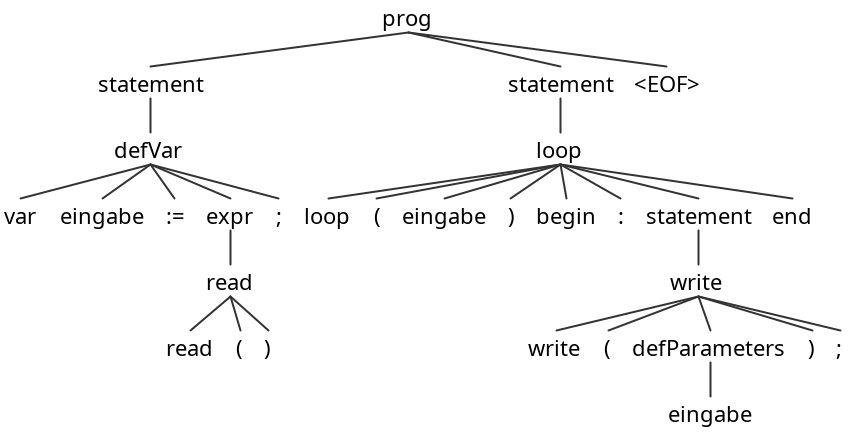
\includegraphics[width=12cm]{content/pictures/ast.png}
	\caption{Ein \acl{ast}}
	%	\source{\cite[S. 5]{SemtechCorporation.2020}}
	\label{pic:isZeroAST}
\end{figure}

Darin ist zu erkennen, dass das Programm (prog) aus drei Knoten besteht: zwei Statements und dem Symbol \ac{eof}, welches immer das letzte (unsichtbare) Zeichen in einer Datei ist. Die beiden Statements bestehen wiederum aus Knoten und diese Knoten können wieder Knoten beinhalten. 

Wie bereits in \cref{sec:while-grammar} genauer erläutert, kann ein Programmcode, welches einer Grammatik entspricht, immer noch Fehler beinhalten. In \cref{chap:semantic} wird der erzeugte \ac{ast} auf weitere Fehler überprüft.